% !TEX root = ../../ctfp-print.tex

\lettrine[lhang=0.17]{N}{owadays you can't} talk about functional programming without mentioning
monads. But there is an alternative universe in which, by chance,
Eugenio Moggi turned his attention to Lawvere theories rather than
monads. Let's explore that universe.

\section{Universal Algebra}

There are many ways of describing algebras at various levels of
abstraction. We try to find a general language to describe things like
monoids, groups, or rings. At the simplest level, all these
constructions define \emph{operations} on elements of a set, plus some
\emph{laws} that must be satisfied by these operations. For instance, a
monoid can be defined in terms of a binary operation that is
associative. We also have a unit element and unit laws. But with a
little bit of imagination we can turn the unit element to a nullary
operation --- an operation that takes no arguments and returns a special
element of the set. If we want to talk about groups, we add a unary
operator that takes an element and returns its inverse. There are
corresponding left and right inverse laws to go with it. A ring defines
two binary operators plus some more laws. And so on.

The big picture is that an algebra is defined by a set of $n$-ary
operations for various values of $n$, and a set of equational identities.
These identities are all universally quantified. The associativity
equation must be satisfied for all possible combinations of three
elements, and so on.

Incidentally, this eliminates fields from consideration, for the simple
reason that zero (unit with respect to addition) has no inverse with
respect to multiplication. The inverse law for a field can't be
universally quantified.

This definition of a universal algebra can be extended to categories
other than $\Set$, if we replace operations (functions) with
morphisms. Instead of a set, we select an object $a$ (called a
generic object). A unary operation is just an endomorphism of
$a$. But what about other arities (\newterm{arity} is the number of
arguments for a given operation)? A binary operation (arity 2) can be
defined as a morphism from the product $a\times{}a$ back to $a$.
A general $n$-ary operation is a morphism from the $n^\text{th}$ power of
$a$ to $a$:
\[\alpha_n \Colon a^n \to a\]
A nullary operation is a morphism from the terminal object (the zeroth
power of $a$). So all we need in order to define any algebra is a
category whose objects are powers of one special object $a$. The
specific algebra is encoded in the hom-sets of this category. This is a
Lawvere theory in a nutshell.

The derivation of Lawvere theories goes through many steps, so here's
the roadmap:

\begin{enumerate}
  \tightlist
  \item
        Category of finite sets $\cat{FinSet}$.
  \item
        Its skeleton $\cat{F}$.
  \item
        Its opposite $\Fop$.
  \item
        Lawvere theory $\cat{L}$: an object in the category $\cat{Law}$.
  \item
        Model $M$ of a Lawvere category: an object in the category\\
        $\cat{Mod}(\cat{Law}, \Set)$.
\end{enumerate}

\begin{figure}[H]
  \centering
  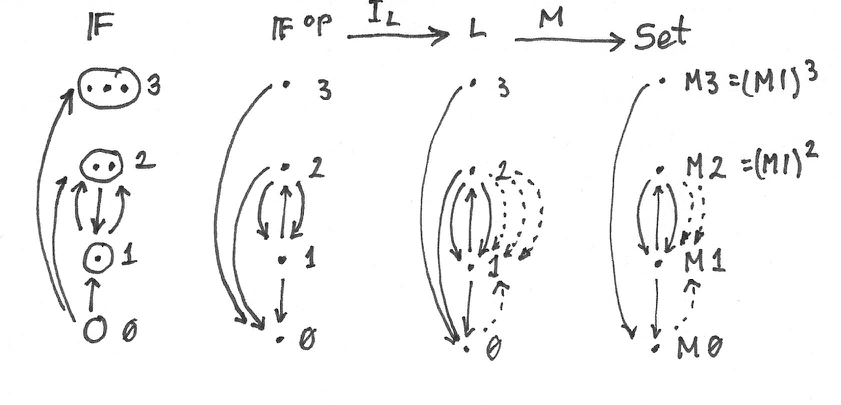
\includegraphics[width=0.8\textwidth]{images/lawvere1.png}
\end{figure}

\section{Lawvere Theories}

All Lawvere theories share a common backbone. All objects in a Lawvere
theory are generated from just one object using products (really, just
powers). But how do we define these products in a general category? It
turns out that we can define products using a mapping from a simpler
category. In fact this simpler category may define coproducts instead of
products, and we'll use a \emph{contravariant} functor to embed them in
our target category. A contravariant functor turns coproducts into
products and injections to projections.

The natural choice for the backbone of a Lawvere category is the
category of finite sets, $\cat{FinSet}$. It contains the empty set
$\varnothing$, a singleton set $1$, a two-element set $2$,
and so on. All objects in this category can be generated from the
singleton set using coproducts (treating the empty set as a special case
of a nullary coproduct). For instance, a two-element set is a sum of two
singletons, $2 = 1 + 1$, as expressed in Haskell:

\src{snippet01}
However, even though it's natural to think that there's only one empty
set, there may be many distinct singleton sets. In particular, the set
$1 + \varnothing$ is different from the set $\varnothing + 1$, and
different from $1$ --- even though they are all isomorphic. The
coproduct in the category of sets is not associative. We can remedy that
situation by building a category that identifies all isomorphic sets.
Such a category is called a \newterm{skeleton}. In other words, the
backbone of any Lawvere theory is the skeleton $\cat{F}$ of
$\cat{FinSet}$. The objects in this category can be identified with
natural numbers (including zero) that correspond to the element count in
$\cat{FinSet}$. Coproduct plays the role of addition. Morphisms in
$\cat{F}$ correspond to functions between finite sets. For instance,
there is a unique morphism from $\varnothing$ to $n$ (empty set
being the initial object), no morphisms from $n$ to $\varnothing$
(except $\varnothing \to \varnothing$), $n$ morphisms from $1$ to
$n$ (the injections), one morphism from $n$ to $1$,
and so on. Here, $n$ denotes an object in $\cat{F}$
corresponding to all $n$-element sets in $\cat{FinSet}$ that have been
identified through isomorphisms.

Using the category $\cat{F}$ we can formally define a \newterm{Lawvere
  theory} as a category $\cat{L}$ equipped with a special functor:
\[I_{\cat{L}} \Colon \Fop \to \cat{L}\]
This functor must be a bijection on objects and it must preserve finite
products (products in $\Fop$ are the same as
coproducts in $\cat{F}$):
\[I_{\cat{L}}\ (m\times{}n) = I_{\cat{L}}\ m\times{}I_{\cat{L}}\ n\]
You may sometimes see this functor characterized as identity-on-objects,
which means that the objects in $\cat{F}$ and $\cat{L}$ are the same.
We will therefore use the same names for them --- we'll denote them by
natural numbers. Keep in mind though that objects in $\cat{F}$ are not
the same as sets (they are classes of isomorphic sets).

The hom-sets in $\cat{L}$ are, in general, richer than those in
$\Fop$. They may contain morphisms other than
the ones corresponding to functions in $\cat{FinSet}$ (the latter are
sometimes called \newterm{basic product operations}). Equational laws of a
Lawvere theory are encoded in those morphisms.

The key observation is that the singleton set $1$ in $\cat{F}$
is mapped to some object that we also call $1$ in $\cat{L}$, and
all the other objects in $\cat{L}$ are automatically powers of this
object. For instance, the two-element set $2$ in $\cat{F}$ is
the coproduct $1 + 1$, so it must be mapped to a product
$1 \times 1$ (or $1^2$) in $\cat{L}$. In this sense, the category
$\cat{F}$ behaves like the logarithm of $\cat{L}$.

Among morphisms in $\cat{L}$ we have those transferred by the functor
$I_{\cat{L}}$ from $\cat{F}$. They play a structural role in $\cat{L}$. In
particular coproduct injections $i_k$ become product projections
$p_k$. A useful intuition is to imagine the projection:
\[p_k \Colon 1^n \to 1\]
as the prototype for a function of $n$ variables that ignores all but the
$k^\text{th}$ variable. Conversely, constant morphisms $n \to 1$
in $\cat{F}$ become diagonal morphisms $1 \to 1^n$ in
$\cat{L}$. They correspond to duplication of variables.

The interesting morphisms in $\cat{L}$ are the ones that define $n$-ary
operations other than projections. It's those morphisms that distinguish
one Lawvere theory from another. These are the multiplications, the
additions, the selections of unit elements, and so on, that define the
algebra. But to make $\cat{L}$ a full category, we also need compound
operations $n \to m$ (or, equivalently,
$1^n \to 1^m$). Because of the simple structure of
the category, they turn out to be products of simpler morphisms of the
type $n \to 1$. This is a generalization of the
statement that a function that returns a product is a product of
functions (or, as we've seen earlier, that the hom-functor is
continuous).

\begin{figure}[H]
  \centering
  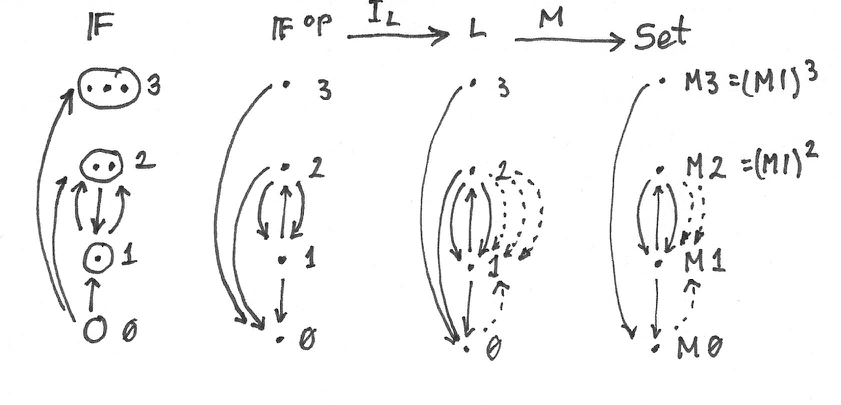
\includegraphics[width=0.8\textwidth]{images/lawvere1.png}
  \caption{Lawvere theory $\cat{L}$ is based on $\Fop$, from which
    it inherits the ``boring'' morphisms that define the products. It adds
    the ``interesting'' morphisms that describe the $n$-ary operations (dotted
    arrows).}
\end{figure}

Lawvere theories form a category $\cat{Law}$, in which morphisms are
functors that preserve finite products and commute with the functors
$I$. Given two such theories, $(\cat{L}, I_{\cat{L}})$ and
$(\cat{L'}, I'_{\cat{L'}})$, a morphism between them is a
functor $F \Colon \cat{L} \to \cat{L'}$ such that:
\begin{gather*}
  F\ (m \times n) = F\ m \times F\ n \\
  F \circ I_{\cat{L}} = I'_{\cat{L'}}
\end{gather*}
Morphisms between Lawvere theories encapsulate the idea of the
interpretation of one theory inside another. For instance, group
multiplication may be interpreted as monoid multiplication if we ignore
inverses.

The simplest trivial example of a Lawvere category is
$\Fop$ itself (corresponding to the choice of
the identity functor for $I_{\cat{L}}$). This Lawvere theory that has no
operations or laws happens to be the initial object in $\cat{Law}$.

At this point it would be very helpful to present a non-trivial example
of a Lawvere theory, but it would be hard to explain it without first
understanding what models are.

\section{Models of Lawvere Theories}

The key to understand Lawvere theories is to realize that one such
theory generalizes a lot of individual algebras that share the same
structure. For instance, the Lawvere theory of monoids describes the
essence of being a monoid. It must be valid for all monoids. A
particular monoid becomes a model of such a theory. A model is defined
as a functor from the Lawvere theory $\cat{L}$ to the category of sets
$\Set$. (There are generalizations of Lawvere theories that use
other categories for models but here I'll just concentrate on
$\Set$.) Since the structure of $\cat{L}$ depends heavily on
products, we require that such a functor preserve finite products. A
model of $\cat{L}$, also called the algebra over the Lawvere theory
$\cat{L}$, is therefore defined by a functor:
\begin{gather*}
  M \Colon \cat{L} \to \Set \\
  M\ (a \times b) \cong M\ a \times M\ b
\end{gather*}
Notice that we require the preservation of products only \emph{up to
  isomorphism}. This is very important, because strict preservation of
products would eliminate most interesting theories.

The preservation of products by models means that the image of
$M$ in $\Set$ is a sequence of sets generated by powers of
the set $M\ 1$ --- the image of the object $1$ from
$\cat{L}$. Let's call this set $a$. (This set is sometimes
called a \emph{sort}, and such an algebra is called \newterm{single-sorted}. There
exist generalizations of Lawvere theories to multi-sorted algebras.) In
particular, binary operations from $\cat{L}$ are mapped to functions:
\[a \times a \to a\]
As with any functor, it's possible that multiple morphisms in $\cat{L}$
are collapsed to the same function in $\Set$.

Incidentally, the fact that all laws are universally quantified
equalities means that every Lawvere theory has a trivial model: a
constant functor mapping all objects to the singleton set, and all morphisms
to the identity function on it.

A general morphism in $\cat{L}$ of the form
$m \to n$ is mapped to a function:
\[a^m \to a^n\]
If we have two different models, $M$ and $N$, a natural
transformation between them is a family of functions indexed by
$n$:
\[\mu_n \Colon M\ n \to N\ n\]
or, equivalently:
\[\mu_n \Colon a^n \to b^n\]
where $b = N\ 1$.

Notice that the naturality condition guarantees the preservation of
$n$-ary operations:
\[N\ f \circ \mu_n = \mu_1 \circ M\ f\]
where $f \Colon n \to 1$ is an $n$-ary operation in
$\cat{L}$.

The functors that define models form a category of models,
$\cat{Mod}(\cat{L}, \Set)$, with natural transformations as morphisms.

Consider a model for the trivial Lawvere category
$\Fop$. Such a model is completely determined by
its value at $1$, $M\ 1$. Since $M\ 1$ can be any
set, there are as many of these models as there are sets in
$\Set$. Moreover, every morphism in $\cat{Mod}(\Fop, \Set)$ (a
natural transformation between functors $M$ and $N$) is
uniquely determined by its component at $M\ 1$. Conversely, every
function $M\ 1 \to N\ 1$ induces a natural
transformation between the two models $M$ and $N$.
Therefore $\cat{Mod}(\Fop, \Set)$ is equivalent to $\Set$.

\section{The Theory of Monoids}

The simplest nontrivial example of a Lawvere theory describes the
structure of monoids. It is a single theory that distills the structure
of all possible monoids, in the sense that the models of this theory
span the whole category $\cat{Mon}$ of monoids. We've already seen a
\hyperref[free-monoids]{universal
  construction}, which showed that every monoid can be obtained from an
appropriate free monoid by identifying a subset of morphisms. So a
single free monoid already generalizes a whole lot of monoids. There
are, however, infinitely many free monoids. The Lawvere theory for
monoids $\cat{L}_{\cat{Mon}}$ combines all of them in one
elegant construction.

Every monoid must have a unit, so we have to have a special morphism
$\eta$ in $\cat{L}_{\cat{Mon}}$ that goes from $0$ to
$1$. Notice that there can be no corresponding morphism in
$\cat{F}$. Such a morphism would go in the opposite direction, from
$1$ to $0$ which, in $\cat{FinSet}$, would be a function
from the singleton set to the empty set. No such function exists.

Next, consider morphisms $2 \to 1$, members of
$\cat{L}_{\cat{Mon}}(2, 1)$, which must contain prototypes of all binary
operations. When constructing models in $\cat{Mod}(\cat{L}_{\cat{Mon}}, \Set)$, these
morphisms will be mapped to functions from the Cartesian product
$M\ 1 \times M\ 1$ to $M\ 1$. In other words, functions of
two arguments.

The question is: how many functions of two arguments can one implement
using only the monoidal operator. Let's call the two arguments
$a$ and $b$. There is one function that ignores both
arguments and returns the monoidal unit. Then there are two projections
that return $a$ and $b$, respectively. They are followed
by functions that return $ab$, $ba$, $aa$,
$bb$, $aab$, and so on\ldots{} In fact there are as many
such functions of two arguments as there are elements in the free monoid
with generators $a$ and $b$. Notice that
$\cat{L}_{\cat{Mon}}(2, 1)$ must contain all those morphisms because one of the
models is the free monoid. In a free monoid they correspond to distinct
functions. Other models may collapse multiple morphisms in
$\cat{L}_{\cat{Mon}}(2, 1)$ down to a single function, but not the free monoid.

If we denote the free monoid with $n$ generators $n^*$, we may
identify the hom-set $\cat{L}(2, 1)$ with the hom-set
$\cat{Mon}(1^*, 2^*)$ in $\cat{Mon}$, the category of monoids. In
general, we pick $\cat{L}_{\cat{Mon}}(m, n)$ to be $\cat{Mon}(n^*, m^*)$. In
other words, the category $\cat{L}_{\cat{Mon}}$ is the opposite of the category
of free monoids.

The category of \emph{models} of the Lawvere theory for monoids,\\
$\cat{Mod}(\cat{L}_{\cat{Mon}}, \Set)$, is equivalent to the category of all monoids,
$\cat{Mon}$.

\section{Lawvere Theories and Monads}

As you may remember, algebraic theories can be described using monads
--- in particular
\hyperref[algebras-for-monads]{algebras
  for monads}. It should be no surprise then that there is a connection
between Lawvere theories and monads.

First, let's see how a Lawvere theory induces a monad. It does it
through an
\hyperref[free-forgetful-adjunctions]{adjunction}
between a forgetful functor and a free functor. The forgetful functor
$U$ assigns a set to each model. This set is given by evaluating
the functor $M$ from $\cat{Mod}(\cat{L}, \Set)$ at the object $1$ in
$\cat{L}$.

Another way of deriving $U$ is by exploiting the fact that
$\Fop$ is the initial object in $\cat{Law}$. It
means that, for any Lawvere theory $\cat{L}$, there is a unique
functor $\Fop \to \cat{L}$. This functor induces the
opposite functor on models (since models are functors \emph{from}
theories to sets):
\[\cat{Mod}(\cat{L}, \Set) \to \cat{Mod}(\Fop, \Set)\]
But, as we discussed, the category of models of
$\Fop$ is equivalent to $\Set$, so we get
the forgetful functor:
\[U \Colon \cat{Mod}(\cat{L}, \Set) \to \Set\]
It can be shown that so defined $U$ always has a left adjoint,
the free functor $F$.

This is easily seen for finite sets. The free functor $F$
produces free algebras. A free algebra is a particular model in
$\cat{Mod}(\cat{L}, \Set)$ that is generated from a finite set of generators
$n$. We can implement $F$ as the representable functor:
\[\cat{L}(n, -) \Colon \cat{L} \to \Set\]
To show that it's indeed free, all we have to do is to prove that it's a
left adjoint to the forgetful functor:
\[\cat{Mod}(\cat{L}(n, -), M) \cong \Set(n, U(M))\]
Let's simplify the right hand side:
\[\Set(n, U(M)) \cong \Set(n, M\ 1) \cong (M\ 1)^n \cong M\ n\]
(I used the fact that a set of morphisms is isomorphic to the
exponential which, in this case, is just the iterated product.) The
adjunction is the result of the Yoneda lemma:
\[[\cat{L}, \Set](\cat{L}(n, -), M) \cong M\ n\]
Together, the forgetful and the free functor define a
\hyperref[monads-categorically]{monad}
$T = U \circ F$ on $\Set$. Thus every Lawvere theory generates
a monad.

It turns out that the category of
\hyperref[algebras-for-monads]{algebras
  for this monad} is equivalent to the category of models.

You may recall that monad algebras define ways to evaluate expressions
that are formed using monads. A Lawvere theory defines n-ary operations
that can be used to generate expressions. Models provide means to
evaluate these expressions.

The connection between monads and Lawvere theories doesn't go both ways,
though. Only finitary monads lead to Lawvere theories. A finitary monad
is based on a finitary functor. A finitary functor on $\Set$ is
fully determined by its action on finite sets. Its action on an
arbitrary set $a$ can be evaluated using the following coend:
\[F\ a = \int^n a^n \times (F\ n)\]
Since the coend generalizes a coproduct, or a sum, this formula is a
generalization of a power series expansion. Or we can use the intuition
that a functor is a generalized container. In that case a finitary
container of $a$s can be described as a sum of shapes and
contents. Here, $F\ n$ is a set of shapes for storing $n$ elements,
and the contents is an $n$-tuple of elements, itself an element of
$a^n$. For instance, a list (as a functor) is finitary, with one
shape for every arity. A tree has more shapes per arity, and so on.

First off, all monads that are generated from Lawvere theories are
finitary and they can be expressed as coends:
\[T_{\cat{L}}\ a = \int^n a^n \times \cat{L}(n, 1)\]
Conversely, given any finitary monad $T$ on $\Set$, we can
construct a Lawvere theory. We start by constructing a Kleisli category
for $T$. As you may remember, a morphism in a Kleisli category
from $a$ to $b$ is given by a morphism in the underlying
category:
\[a \to T\ b\]
When restricted to finite sets, this becomes:
\[m \to T\ n\]
The category opposite to this Kleisli category,
$\cat{Kl}^{op}_{T}$, restricted to finite
sets, is the Lawvere theory in question. In particular, the hom-set
$\cat{L}(n, 1)$ that describes n-ary operations in $\cat{L}$ is given
by the hom-set $\cat{Kl}_{T}(1, n)$.

It turns out that most monads that we encounter in programming are
finitary, with the notable exception of the continuation monad. It is
possible to extend the notion of Lawvere theory beyond finitary
operations.

\section{Monads as Coends}

Let's explore the coend formula in more detail.
\[T_{\cat{L}}\ a = \int^n a^n \times \cat{L}(n, 1)\]
To begin with, this coend is taken over a profunctor $P$ in
$\cat{F}$ defined as:
\[P\ n\ m = a^n \times \cat{L}(m, 1)\]
This profunctor is contravariant in the first argument, $n$.
Consider how it lifts morphisms. A morphism in $\cat{FinSet}$ is a
mapping of finite sets $f \Colon m \to n$. Such a
mapping describes a selection of $m$ elements from an $n$-element set
(repetitions are allowed). It can be lifted to the mapping of powers of
$a$, namely (notice the direction):
\[a^n \to a^m\]
The lifting simply selects $m$ elements from a tuple of $n$ elements\\
$(a_1, a_2,...a_n)$ (possibly with repetitions).

\begin{figure}[H]
  \centering
  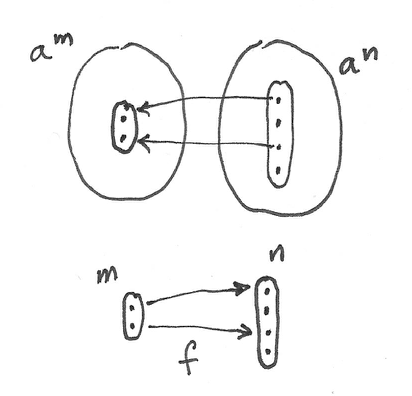
\includegraphics[width=0.5\textwidth]{images/liftpower.png}
\end{figure}

\noindent
For instance, let's take $f_k \Colon 1 \to n$ --- a
selection of the $k^\text{th}$ element from an $n$-element set. It lifts to
a function that takes a $n$-tuple of elements of $a$ and returns
the $k^\text{th}$ one.

Or let's take $f \Colon m \to 1$ --- a constant
function that maps all $m$ elements to one. Its lifting is a function that
takes a single element of $a$ and duplicates it $m$ times:
\[\lambda{}x \to (\underbrace{x, x,\ ...\ , x}_{m})\]
You might notice that it's not immediately obvious that the profunctor
in question is covariant in the second argument. The hom-functor
$\cat{L}(m, 1)$ is actually contravariant in $m$. However, we
are taking the coend not in the category $\cat{L}$ but in the category
$\cat{F}$. The coend variable $n$ goes over finite sets (or the
skeletons of such). The category $\cat{L}$ contains the opposite of
$\cat{F}$, so a morphism $m \to n$ in $\cat{F}$
is a member of $\cat{L}(n, m)$ in $\cat{L}$ (the embedding is given
by the functor $I_{\cat{L}}$).

Let's check the functoriality of $\cat{L}(m, 1)$ as a functor from
$\cat{F}$ to $\Set$. We want to lift a function
$f \Colon m \to n$, so our goal is to implement a
function from $\cat{L}(m, 1)$ to $\cat{L}(n, 1)$. Corresponding to
the function $f$ there is a morphism in $\cat{L}$ from
$n$ to $m$ (notice the direction). Precomposing this
morphism with $\cat{L}(m, 1)$ gives us a subset of
$\cat{L}(n, 1)$.

\begin{figure}[H]
  \centering
  \begin{tikzcd}[column sep=large]
    \cat{L}(m, 1) \arrow[r] & \cat{L}(n, 1)\\
    {}^m \bullet \arrow[r, "f"'] & \bullet^n
  \end{tikzcd}
\end{figure}

\noindent
Notice that, by lifting a function $1 \to n$ we can go
from $\cat{L}(1, 1)$ to $\cat{L}(n, 1)$. We'll use this fact later
on.

The product of a contravariant functor $a^n$ and a covariant
functor $\cat{L}(m, 1)$ is a profunctor
$\Fop \times \cat{F} \to \Set$. Remember that a coend can be defined
as a coproduct (disjoint sum) of all the diagonal members of a
profunctor, in which some elements are identified. The identifications
correspond to cowedge conditions.

Here, the coend starts as the disjoint sum of sets
$a^n \times \cat{L}(n, 1)$ over all $n$s. The identifications can
be generated by expressing the
\hyperref[ends-and-coends]{coend as
  a coequalizer}. We start with an off-diagonal term
$a^n \times \cat{L}(m, 1)$. To get to the diagonal, we can apply a
morphism $f \Colon m \to n$ either to the first or
the second component of the product. The two results are then
identified.

\begin{figure}[H]
  \centering
  \begin{tikzcd}
    & a^n \times \cat{L}(m, 1)
    \arrow[dl, "\langle f {,} \id \rangle"']
    \arrow[dr, "\langle \id {,} f \rangle"]
    & \\
    a^m \times \cat{L}(m, 1)
    & \scalebox{2.5}[1]{\sim}
    & a^n \times \cat{L}(n, 1) \\
    & f \Colon m \to n &
  \end{tikzcd}
\end{figure}

\noindent
I have shown before that the lifting of
$f \Colon 1 \to n$ results in these two
transformations:
\[a^n \to a\]
and:
\[\cat{L}(1, 1) \to \cat{L}(n, 1)\]
Therefore, starting from $a^n \times \cat{L}(1, 1)$ we can reach both:
\[a \times \cat{L}(1, 1)\]
when we lift $\langle f, \id \rangle$ and:
\[a^n \times \cat{L}(n, 1)\]
when we lift $\langle \id, f \rangle$. This doesn't
mean, however, that all elements of $a^n \times \cat{L}(n, 1)$ can be
identified with $a \times \cat{L}(1, 1)$. That's because not all elements
of $\cat{L}(n, 1)$ can be reached from $\cat{L}(1, 1)$. Remember
that we can only lift morphisms from $\cat{F}$. A non-trivial $n$-ary
operation in $\cat{L}$ cannot be constructed by lifting a morphism
$f \Colon 1 \to n$.

In other words, we can only identify all addends in the coend formula
for which $\cat{L}(n, 1)$ can be reached from $\cat{L}(1, 1)$
through the application of basic morphisms. They are all equivalent to
$a \times \cat{L}(1, 1)$. Basic morphisms are the ones that are images of
morphisms in $\cat{F}$.

Let's see how this works in the simplest case of the Lawvere theory, the
$\Fop$ itself. In such a theory, every
$\cat{L}(n, 1)$ can be reached from $\cat{L}(1, 1)$. This is because
$\cat{L}(1, 1)$ is a singleton containing just the identity morphism,
and $\cat{L}(n, 1)$ only contains morphisms corresponding to
injections $1 \to n$ in $\cat{F}$, which \emph{are}
basic morphisms. Therefore all the addends in the coproduct are
equivalent and we get:
\[T\ a = a \times \cat{L}(1, 1) = a\]
which is the identity monad.

\section{Lawvere Theory of Side Effects}

Since there is such a strong connection between monads and Lawvere
theories, it's natural to ask the question if Lawvere theories could be
used in programming as an alternative to monads. The major problem with
monads is that they don't compose nicely. There is no generic recipe for
building monad transformers. Lawvere theories have an advantage in this
area: they can be composed using coproducts and tensor products. On the
other hand, only finitary monads can be easily converted to Lawvere
theories. The outlier here is the continuation monad. There is ongoing
research in this area (see bibliography).

To give you a taste of how a Lawvere theory can be used to describe side
effects, I'll discuss the simple case of exceptions that are
traditionally implemented using the \code{Maybe} monad.

The \code{Maybe} monad is generated by the Lawvere theory with a
single nullary operation $0 \to 1$. A model of this
theory is a functor that maps $1$ to some set $a$, and
maps the nullary operation to a function:

\src{snippet02}
We can recover the \code{Maybe} monad using the coend formula. Let's
consider what the addition of the nullary operation does to the hom-sets
$\cat{L}(n, 1)$. Besides creating a new $\cat{L}(0, 1)$ (which is
absent from $\Fop$), it also adds new morphisms
to $\cat{L}(n, 1)$. These are the results of composing morphism of the
type $n \to 0$ with our $0 \to 1$.
Such contributions are all identified with $a^0 \times \cat{L}(0, 1)$ in
the coend formula, because they can be obtained from:
\[a^n \times \cat{L}(0, 1)\]
by lifting $0 \to n$ in two different ways.

\begin{figure}[H]
  \centering
  \begin{tikzcd}
    & a^n \times \cat{L}(0, 1)
    \arrow[dl, "\langle f {,} \id \rangle"']
    \arrow[dr, "\langle \id {,} f \rangle"]
    & \\
    a^0 \times \cat{L}(0, 1)
    & \scalebox{2.5}[1]{\sim}
    & a^n \times \cat{L}(n, 1) \\
    & f \Colon 0 \to n &
  \end{tikzcd}
\end{figure}

\noindent
The coend reduces to:
\[T_{\cat{L}}\ a = a^0 + a^1\]
or, using Haskell notation:

\src{snippet03}
which is equivalent to:

\src{snippet04}
Notice that this Lawvere theory only supports the raising of exceptions,
not their handling.

\section{Challenges}

\begin{enumerate}
  \tightlist
  \item
        Enumerate all morphisms between $2$ and $3$ in $\cat{F}$ (the skeleton of
        $\cat{FinSet}$).
  \item
        Show that the category of models for the Lawvere theory of monoids is
        equivalent to the category of monad algebras for the list monad.
  \item
        The Lawvere theory of monoids generates the list monad. Show that its
        binary operations can be generated using the corresponding Kleisli
        arrows.
  \item
        \textbf{FinSet} is a subcategory of $\Set$ and there is a
        functor that embeds it in $\Set$. Any functor on $\Set$
        can be restricted to $\cat{FinSet}$. Show that a finitary functor is
        the left Kan extension of its own restriction.
\end{enumerate}

\section{Further Reading}
\begin{enumerate}
  \tightlist
  \item
        \urlref{http://www.tac.mta.ca/tac/reprints/articles/5/tr5.pdf}{Functorial Semantics of Algebraic Theories}, F. William Lawvere
  \item
        \urlref{http://homepages.inf.ed.ac.uk/gdp/publications/Comp_Eff_Monads.pdf}{Notions of computation determine monads}, Gordon Plotkin and John Power
\end{enumerate}
